\section{Nulové body a póly}
Póly a nuly byli získány pomocí funkce "signal.sos2zpk" z dat filtrů a tyto hodnoty byli vykresleny do grafů podle příkladů z \url{https://nbviewer.org/github/zmolikova/ISS_project_study_phase/blob/master/Zvuk_spektra_filtrace.ipynb}.
Navíc byli přidány grafy s detailem na vykreslené body vzhledem k tomu, že tyto body byli tak blízko u sebe že je z nepřiblíženého grafu nelze od sebe skoro rozeznat.

\begin{figure}[H] 
	\centering
	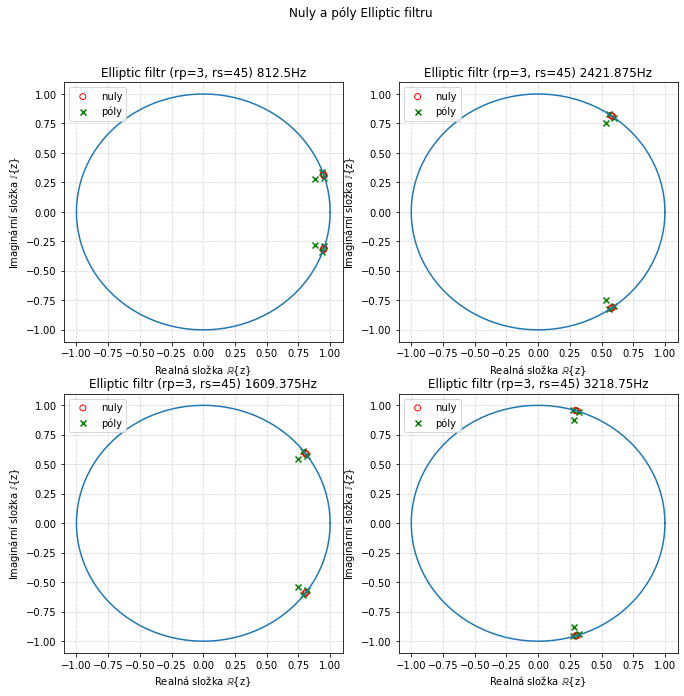
\includegraphics[scale=0.60,keepaspectratio]{Figure_19}
	\caption{Nulové body a póly Elliptic filtrů}
\end{figure}

\begin{figure}[H] 
	\centering
	\includegraphics[scale=0.60,keepaspectratio]{Figure_32}
	\caption{Nulové body a póly Elliptic filtrů (detail)}
\end{figure}

\begin{figure}[H] 
	\centering
	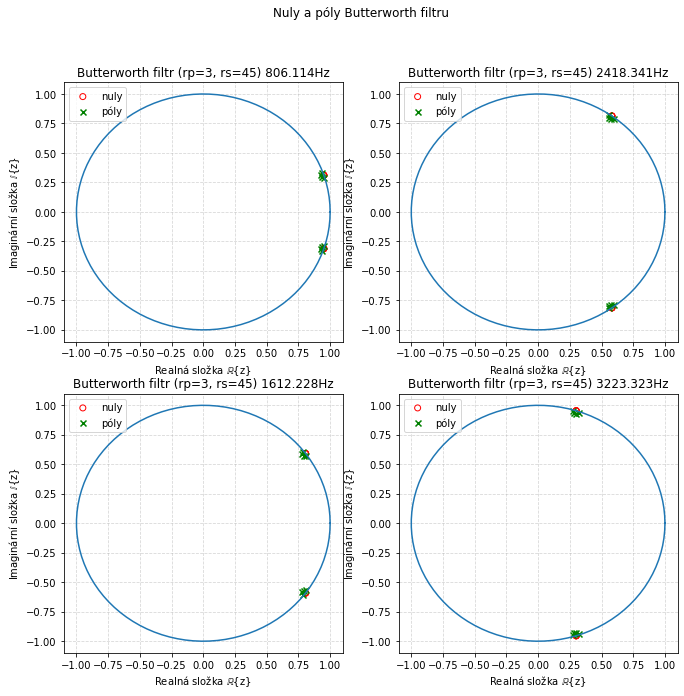
\includegraphics[scale=0.60,keepaspectratio]{Figure_18}
	\caption{Nulové body a póly Butterworthových filtrů}
\end{figure}

\begin{figure}[H] 
	\centering
	\includegraphics[scale=0.6,keepaspectratio]{Figure_31}
	\caption{Nulové body a póly Butterworthových filtrů (detail)}
\end{figure}